\documentclass[addpoints]{exam}

\usepackage{amsmath}
\usepackage{hyperref}
\usepackage{tikz}

% Header and footer.
\pagestyle{headandfoot}
\runningheadrule
\runningfootrule
\runningheader{CS 201 DS II}{Homework 3}{Spring 2018}
\runningfooter{}{Page \thepage\ of \numpages}{}
\firstpageheader{}{}{}

\qformat{{\large\bf Exercise \thequestiontitle}\hfill[\totalpoints\ points]}
\boxedpoints
\printanswers

\title{Habib University\\CS 201 Data Structures II\\Spring 2018}
\author{Don't Grade Me}  % replace with your ID, e.g. sh01703
\date{Homework 3\\Due: 19h; Monday, 23 Feb}

\begin{document}
\maketitle

\begin{questions}

  \titledquestion{12.4}[5]
  Let $G$ be an undirected graph. We say $G$ is {\it connected} if, for every pair of vertices $i$ and $j$ in $G$, there is a path from $i$ to $j$ (since $G$ is undirected, there is also a path from $j$ to $i$). Show how to test if $G$ is connected in $O(n + m)$ time.
  \begin{solution}
    % Write your solution here
  \end{solution}

  \titledquestion{12.5}[5]
  Let $G$ be an undirected graph. A {\it connected-component labelling} of $G$ partitions the vertices of $G$ into maximal sets, each of which forms a connected subgraph. Show how to compute a connected component labelling of $G$ in $O(n + m)$ time.
  \begin{solution}
    % Write your solution here
  \end{solution}

  \titledquestion{12.7}[10]
  We say that a directed graph $G$ is {\it strongly-connected} if, for every pair of vertices $i$ and $j$ in $G$,there is a path from $i$ to $j$. Show how to test if $G$ is strongly-connected in $O(n + m)$ time.
  \begin{solution}
    % Write your solution here
  \end{solution}

  \titledquestion{12.10*}[15]
  A {\it universal sink} in a graph $G$ is a vertex that is the target of $n−1$ edges and the source of no edges.\footnote{A universal sink, $v$, is also sometimes called a {\it celebrity}: Everyone in the room recognizes $v$, but $v$ doesn’t recognize anyone else in the room.} Design an algorithm that tests if a graph $G$, represented as an AdjacencyMatrix, has a universal sink. Your algorithm should run in $O(n)$ time.\\
  \underline{Hint}: Draw a few graphs with a universal sink and observe their adjacency matrix.
  \begin{solution}
    % Write your solution here
  \end{solution}

  \qformat{{\large\bf \thequestiontitle}\hfill[\totalpoints\ points]}

  \titledquestion{Graph Complement}[15]

  The complement of an undirected graph $G$ is a graph $H$ on the same vertices such that two distinct vertices of $H$ are adjacent (connected by an edge) if and only if they are not adjacent in $G$.\footnote{\url{https://en.wikipedia.org/wiki/Complement_graph}} Prove that if $G$ is not a connected graph then its complement $H$ is a connected graph.
  \begin{solution}
    % Write your solution here
  \end{solution}

  \titledquestion{Topological Sort}[15]

  A {\it topological sort} or {\it topological ordering} of a directed graph is a linear ordering of its vertices such that for every directed edge $(u,v)$ from vertex $u$ to vertex $v$, $u$ comes before $v$ in the ordering.\footnote{\url{https://en.wikipedia.org/wiki/Topological_sorting}}

  Find a topological ordering of each of the following two graphs.

  \begin{parts}
    \part[5]
    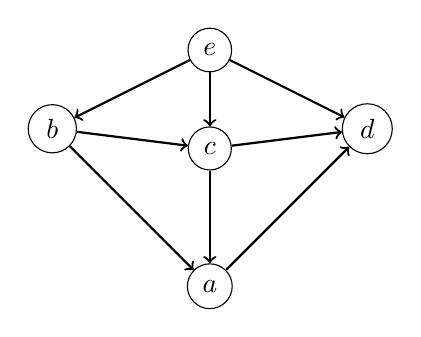
\begin{tikzpicture}
      \foreach \pos/\name in { {(2,0)/a}, {(0,2)/b}, {(2,1.75)/c}, {(4,2)/d}, {(2,3)/e}}
      \node[circle,draw] (\name) at \pos {$\name$};
      \foreach \source/ \dest in {a/d, c/d, c/a, b/a, b/c, e/b, e/c, e/d}
      \path[draw,thick,->] (\source) -- (\dest);
    \end{tikzpicture}
    \begin{solution}
      % Write your solution here
    \end{solution}
    \part[10]

    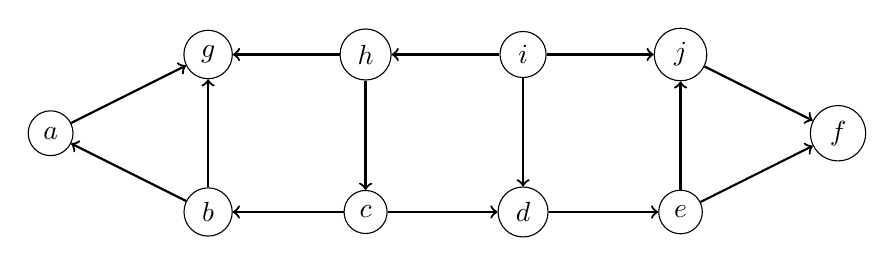
\begin{tikzpicture}
      \foreach \pos/\name in {{(0,1)/a}, {(2,0)/b}, {(4,0)/c}, {(6,0)/d}, {(8,0)/e}, {(10,1)/f}, {(2,2)/g}, {(4,2)/h}, {(6,2)/i}, {(8,2)/j}}
      \node[circle,draw] (\name) at \pos {$\name$};
      \foreach \source/ \dest in {b/a, a/g, b/g, c/b, c/d, d/e, e/f, e/j, h/g, i/h, h/c, i/d, i/j, j/f}
      \path[draw,thick,->] (\source) -- (\dest);
    \end{tikzpicture}
    \begin{solution}
      % Write your solution here
    \end{solution}
  \end{parts}
  
\end{questions}

* - The question has been modified from the one in the book.

\end{document}